\documentclass[10pt,journal,compsoc]{IEEEtran}

\ifCLASSOPTIONcompsoc
  \usepackage[nocompress]{cite}
  \usepackage{tabularx}
  \usepackage{array}
  \usepackage{hyperref}
  \usepackage{graphicx}
  \usepackage{caption}
 \usepackage[numbers]{natbib}
\bibliographystyle{plainnat}
\else
  % normal IEEE
  \usepackage{cite}
\fi


% *** GRAPHICS RELATED PACKAGES ***
%
\ifCLASSINFOpdf
\else

\fi
\newcommand\MYhyperrefoptions{bookmarks=true,bookmarksnumbered=true,
pdfpagemode={UseOutlines},plainpages=false,pdfpagelabels=true,
colorlinks=true,linkcolor={black},citecolor={black},urlcolor={black},
pdftitle={Bare Demo of IEEEtran.cls for Computer Society Journals},%<!CHANGE!
pdfsubject={Typesetting},%<!CHANGE!
pdfauthor={Michael D. Shell},%<!CHANGE!
pdfkeywords={Computer Society, IEEEtran, journal, LaTeX, paper,
             template}}%<^!CHANGE!

\hyphenation{optical networks semiconductor}


\begin{document}
\title{Visualización de datos: Caso Cáncer Pulmonar}


\author{Jose Edison~Perez Mamani,
        and~Henrry Ivan~Arias Mamani% <-this % stops a space
}


\IEEEtitleabstractindextext{%
\begin{abstract}
El cáncer pulmonar sigue siendo una de las principales causas de mortalidad global debido a su diagnóstico tardío y a la baja tasa de supervivencia a cinco años. A pesar de los avances en tratamientos, la identificación temprana y el tratamiento personalizado siguen siendo un reto significativo. Este artículo explora cómo la ciencia de datos puede mejorar la comprensión de la enfermedad mediante el análisis de grandes volúmenes de datos clínicos y genómicos. Utilizando técnicas avanzadas como el PCA y  t-SNE, se busca identificar patrones y correlaciones que puedan contribuir a mejorar el diagnóstico.

El estudio se enfoca en analizar factores demográficos y médicos que afectan la supervivencia de los pacientes con cáncer pulmonar, como la edad, el género, el estado de tabaquismo y el índice de masa corporal. El objetivo principal es llenar el vacío existente en la comprensión de cómo estos factores influyen en el tratamiento y la mortalidad de los pacientes. El artículo propone un análisis detallado que busca mejorar  la tasa de supervivencia mediante la identificación de patrones y correlaciones en los datos.
\end{abstract}

% Note that keywords are not normally used for peerreview papers.
\begin{IEEEkeywords}
Lung cancer, PCA, visualization analysis, T-SNE.
\end{IEEEkeywords}

}

% make the title area
\maketitle
\IEEEdisplaynontitleabstractindextext

\IEEEpeerreviewmaketitle


\ifCLASSOPTIONcompsoc
\IEEEraisesectionheading{\section{Introduction}\label{sec:introduction}}
\else
\section{Introduction}
\label{sec:introduction}
\fi

\IEEEPARstart{E}{l} El cáncer pulmonar es una de las principales causas de mortalidad a nivel mundial, con un pronóstico a menudo desfavorable debido a la detección tardía de la enfermedad. A pesar de los avances en la oncología y los tratamientos personalizados, la tasa de supervivencia a cinco años sigue siendo baja. La ciencia de datos ha emergido como una herramienta poderosa para abordar los desafíos en la detección temprana, diagnóstico y personalización del tratamiento en cáncer pulmonar. Mediante el uso de técnicas avanzadas, es posible analizar grandes volúmenes de datos clínicos y genómicos para identificar patrones y desarrollar modelos predictivos que puedan mejorar los resultados para los pacientes .

\subsection{Objetivo}
El principal objetivo de este artículo es identificar y analizar los factores demográficos y médicos que influencian la supervivencia de los pacientes con cáncer de pulmón. En particular, el artículo intente evaluarse cómo las variables tales como la edad, el género, el estado de tabaquismo, el índice de masa corporal, el nivel de colesterol, la historia familiar acerca de cáncer, y la etapa del cáncer en el momento del diagnóstico afectan el tratamiento y los resultados de los pacientes.

\subsection{Problema}
A pesar de los avances realizados en el tratamiento de del cáncer de pulmón, el índice de mortalidad continúa siendo elevado. El problema que pretende abordar este articulo radica en la falta de comprensión detallada acerca de cómo varios de factores demográficos, médicos y terapéuticos influyen en la supervivencia de los pacientes con cáncer de pulmón. Aunque existe una serie de estudios previos que exploran sobre este tema, la complejidad de la interrelación entre varios factores, sus afectos al tratamiento y la supervivencia no ha sido suficientemente explorada. Este articulo intenta llenar este vacío ofreciendo un análisis a fondo de varios factores relacionados con la mortalidad de los pacientes que sufren de cáncer de pulmón y proporcionando la base para la mejora de las estrategias de tratamiento. Con la ayuda de este enfoque, podrás centrar tu análisis en la identificación de patrones y correlaciones que puedan ser útiles para la mejora de enfoques terapéuticos y, como resultado, de las tasas de supervivencia.


\section{Trabajos relacionados}

En el articulo \cite{ferraz2017}, se investigó la influencia de factores pronósticos como la edad, el estadiamiento y la extensión del tumor en la supervivencia de mujeres con cáncer de mama, utilizando modelos de riesgos proporcionales de Cox y riesgos competitivos de Fine-Gray. Se analizaron los datos de una cohorte retrospectiva de 524 mujeres en Campinas, Brasil, diagnosticadas entre 1993 y 1995. Se aplicaron estos modelos para evaluar la influencia de los factores mencionados en la mortalidad específica por cáncer de mama y otras causas competidoras. Las curvas de supervivencia estimadas por Kaplan-Meier mostraron diferencias significativas en las muertes por cáncer de mama y por riesgos competidores, aunque la edad no fue un factor significativo en ninguno de los modelos.

El uso de los modelos de Cox y Fine-Gray como muestra \cite{ferraz2017} ofrece ventajas al permitir una estimación más precisa de los riesgos asociados al cáncer de mama y otras causas de muerte. Mientras que los modelos de Cox son útiles para evaluar el impacto de las covariables en la supervivencia, el modelo de Fine-Gray permite considerar la presencia de riesgos competidores, lo que ofrece una visión más realista del escenario clínico. Sin embargo, una desventaja es que la complejidad de estos modelos puede dificultar su interpretación y aplicación práctica en ciertos contextos. Además, aunque ambos modelos identificaron factores pronósticos similares, la ausencia de significancia de la edad en estos análisis sugiere que otros factores podrían ser más determinantes en la supervivencia de estas pacientes.

En el articulo \cite{arxiv14031949}, se implementado una combinación de Análisis de Componentes Principales (PCA) y la técnica de remuestreo Synthetic Minority Over-sampling Technique (SMOTE) para mejorar la precisión en la predicción en un conjunto de datos sobre cáncer de pulmón. PCA se utilizó inicialmente para reducir la dimensionalidad del conjunto de datos, comprimiendo el espacio de características y eliminando atributos redundantes e irrelevantes. Posteriormente, aplicamos SMOTE para equilibrar la distribución de clases, generando nuevas muestras sintéticas en la clase minoritaria. Esta combinación metodológica no solo facilita un modelo de clasificación más eficiente, sino que también incrementa la diversidad del dominio de las muestras, mejorando así el rendimiento del clasificador Naïve Bayes aplicado en la etapa final.

Los resultados obtenidos en el articulo  \cite{arxiv14031949} confirman la eficacia de la metodología propuesta, mostrando mejoras significativas en varias métricas de evaluación, incluyendo la precisión global, la tasa de falsos positivos, la precisión y el recall. En particular, se observó que la aplicación secuencial de PCA seguida por SMOTE permitió una mejora considerable en la exactitud del modelo, aumentando de un 60$\%$ a más del 80$\%$ después de las iteraciones de SMOTE. Estos hallazgos sugieren que la combinación de técnicas de reducción de dimensionalidad y remuestreo puede ser una estrategia efectiva para abordar problemas de desequilibrio de clases y características redundantes en conjuntos de datos médicos.


\begin{figure}[htb]
    \centering
    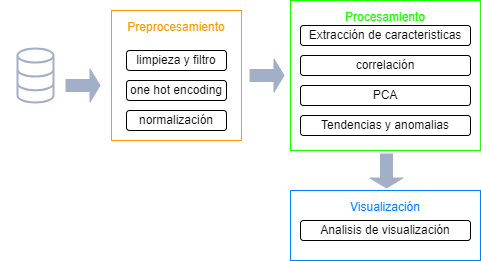
\includegraphics[width=\linewidth]{imagenes/pipeline.png} % Asegúrate de que "pipeline.png" exista en la carpeta "imagenes"
    \caption{Descripción general de pipeline de la propuesta para diagnosticar cancer pulmonar}
    \label{fig:pipeline}
\end{figure}


\begin{figure}[htb]
    \centering
    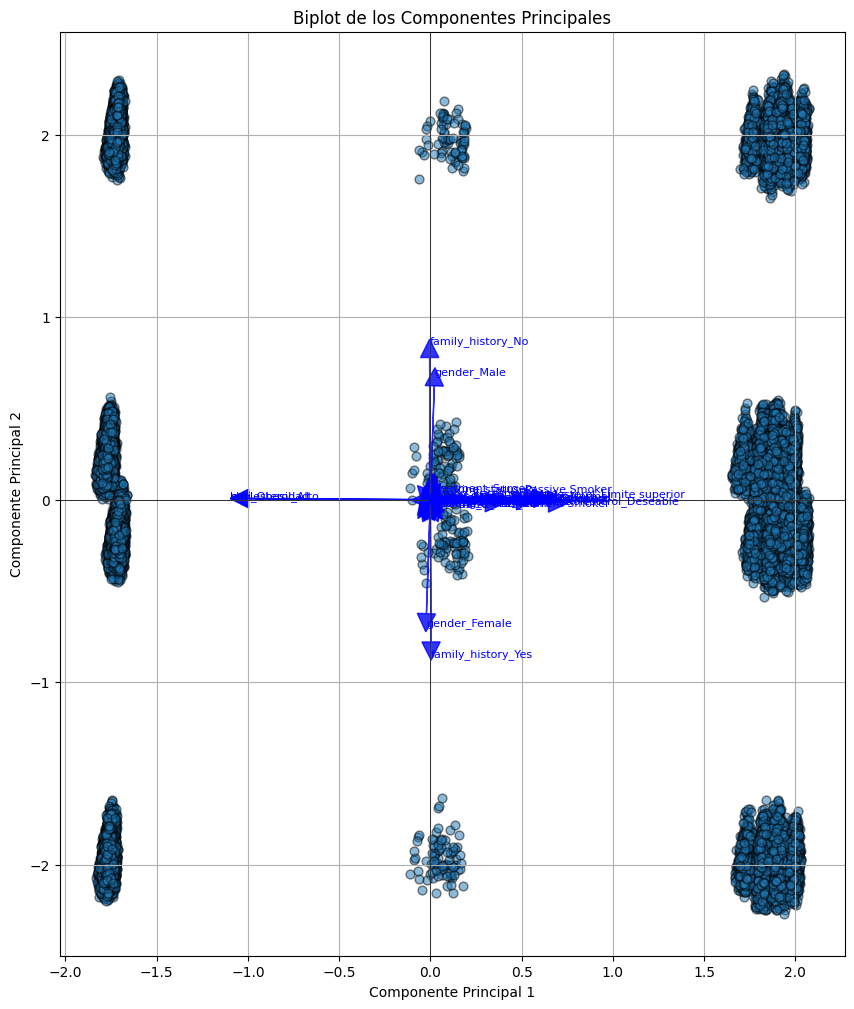
\includegraphics[width=\linewidth]{imagenes/pca_biplot.png}
    \caption{Resultado de la aplicación de PCA para reducir las variables a dos. Los vectores muestran el peso de cada variable por componente.}
    \label{fig:pca}
\end{figure}

\begin{figure}[htb]
    \centering
    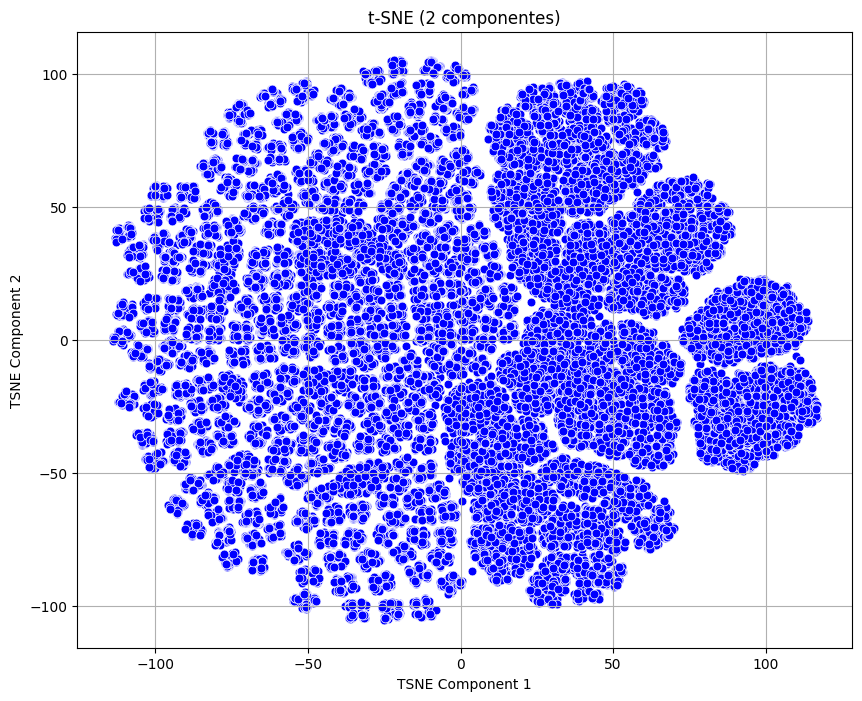
\includegraphics[width=\linewidth]{imagenes/tsne.png}
    \caption{Resultado de la aplicación de t-SNE. Se pueden apreciar agrupaciones de características.}
    \label{fig:tsne}
\end{figure}

\begin{figure}[htb]
    \centering
    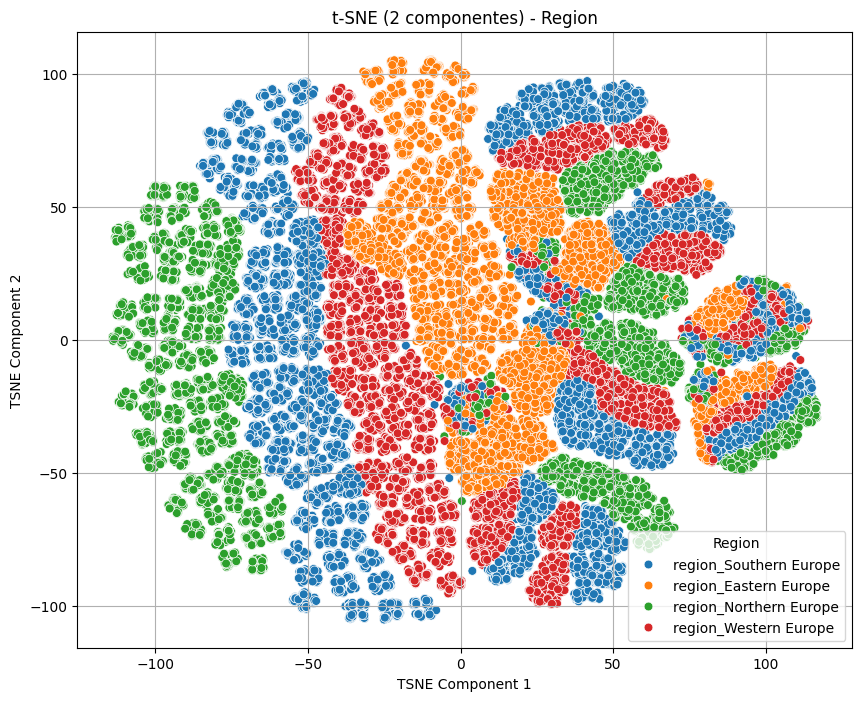
\includegraphics[width=\linewidth]{imagenes/region.png}
    \caption{Clusters según la región de Europa}
    \label{fig:tsne_region}
\end{figure}

\begin{figure}[htb]
    \centering
    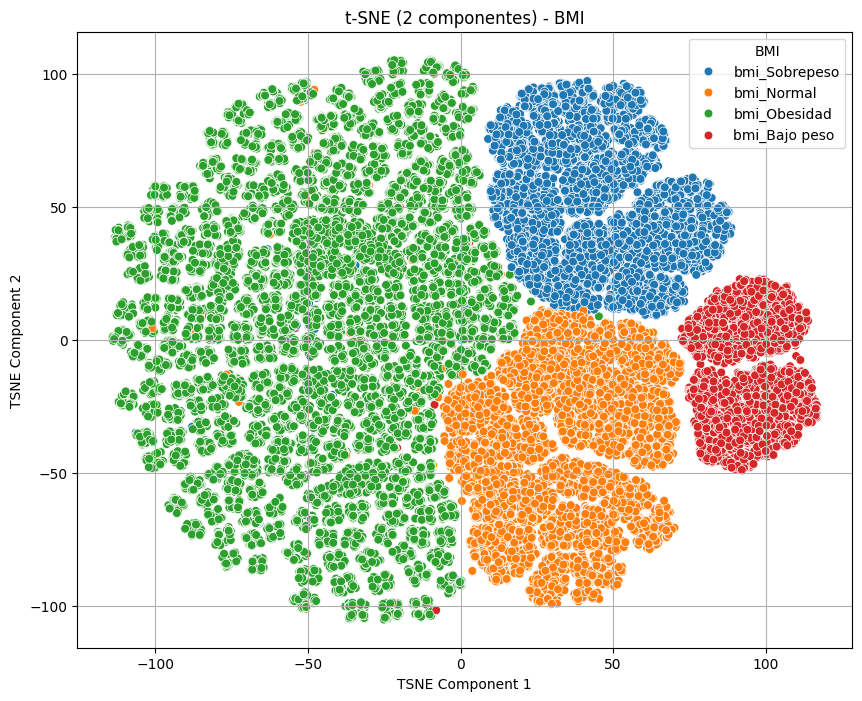
\includegraphics[width=\linewidth]{imagenes/bmi.png}
    \caption{Clusters de acuerdo al índice de masa corporal (BMI)}
    \label{fig:tsne_bmi}
\end{figure}

\begin{figure}[htb]
    \centering
    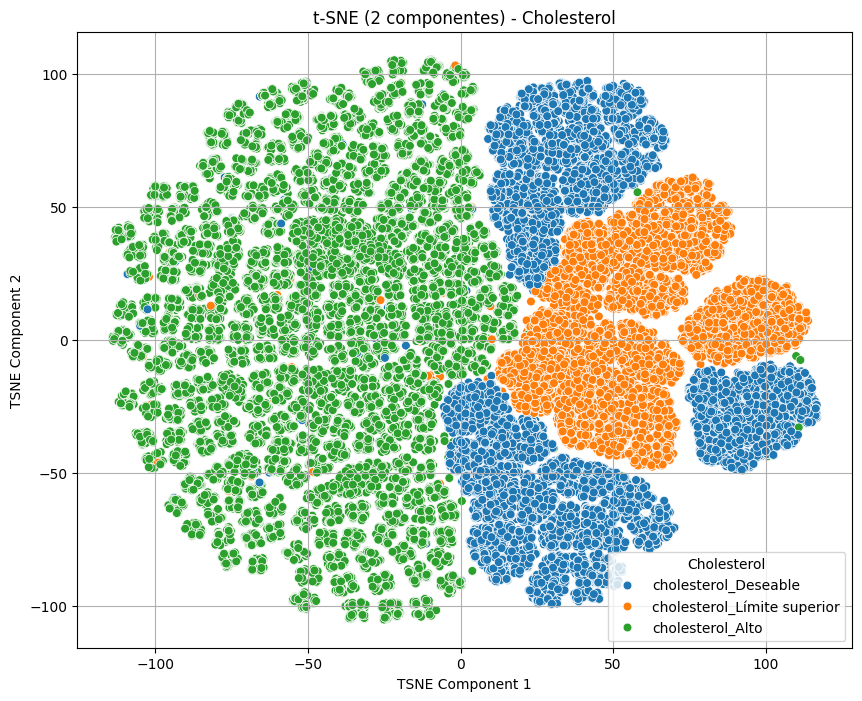
\includegraphics[width=\linewidth]{imagenes/cholesterol.png}
    \caption{Clusters de acuerdo al nivel de colesterol}
    \label{fig:tsne_cholesterol}
\end{figure}

\begin{figure}[htb]
    \centering
    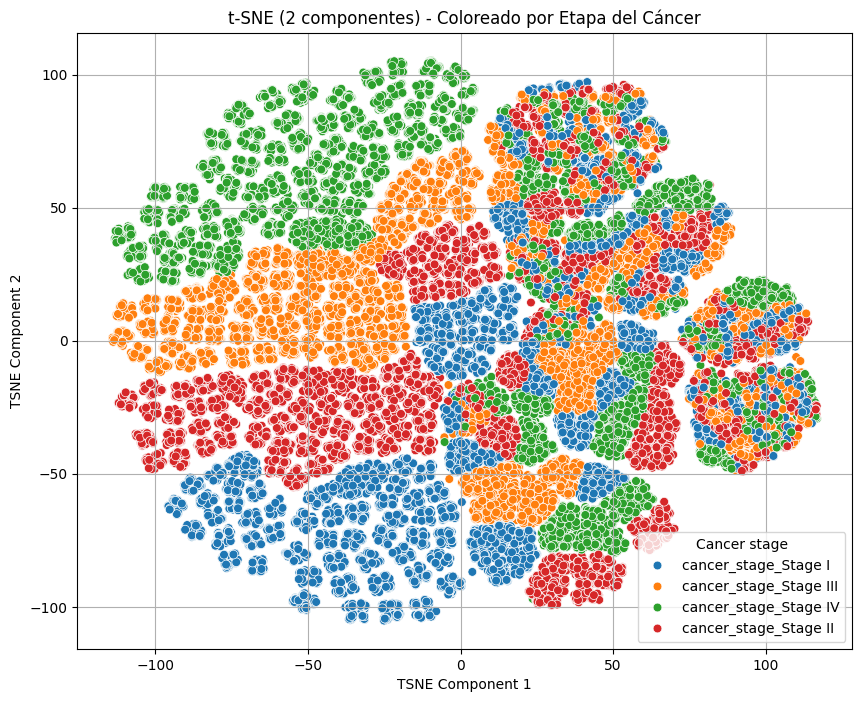
\includegraphics[width=\linewidth]{imagenes/cancer_stage.png}
    \caption{Clusters de acuerdo a la etapa diagnosticada de cáncer}
    \label{fig:tsne_cancer_stage}
\end{figure}

\begin{figure}[htb]
    \centering
    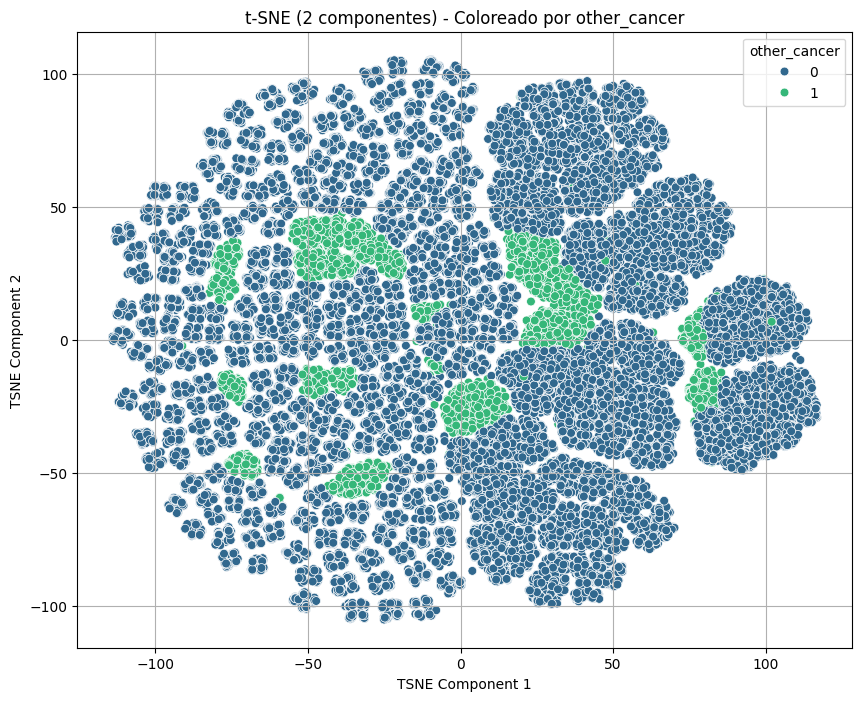
\includegraphics[width=\linewidth]{imagenes/other_cancer.png}
    \caption{Clusters de acuerdo a la presencia o no de otros tipos de cáncer}
    \label{fig:tsne_other_cancer}
\end{figure}


\section{Marco Teórico}
El Análisis de Componentes Principales (PCA, por sus siglas en inglés) es una técnica estadística de reducción de dimensionalidad utilizada para transformar un conjunto de variables posiblemente correlacionadas en un conjunto de variables no correlacionadas, conocidas como componentes principales. Cada componente principal es una combinación lineal de las variables originales, capturando la mayor variabilidad posible en los datos. PCA se basa en el cálculo de vectores propios y valores propios de la matriz de covarianza del conjunto de datos, donde los vectores propios determinan la dirección de las nuevas dimensiones y los valores propios indican la cantidad de varianza capturada por cada componente. Esta técnica es especialmente útil en aplicaciones con datos de alta dimensionalidad, como el análisis de imágenes y genética, al reducir el número de dimensiones y mejorar el rendimiento de los modelos predictivos \cite{jolliffe2016pca}.

t-Distributed Stochastic Neighbor Embedding (t-SNE) es una técnica de reducción de dimensionalidad no lineal que se utiliza principalmente para la visualización de datos de alta dimensionalidad. A diferencia de técnicas como PCA, que conservan la variabilidad global de los datos, t-SNE se enfoca en preservar las relaciones locales, es decir, la proximidad entre puntos en el espacio original. Lo hace al modelar las distancias entre pares de puntos usando distribuciones de probabilidad tanto en el espacio original como en el espacio de menor dimensión, y luego minimizando la divergencia de Kullback-Leibler entre estas distribuciones. Esto permite que t-SNE revele estructuras complejas y patrones ocultos en los datos que pueden ser difíciles de discernir con otras técnicas de reducción de dimensionalidad. Es ampliamente utilizado en la visualización de conjuntos de datos en áreas como la genética, la visión por computadora y el procesamiento del lenguaje natural \cite{maaten2008tsne}.


\begin{table}[h!]
\centering
\begin{tabularx}{\columnwidth}{|l|X|}
\hline
\textbf{Tipo de variable}       & \textbf{Atributo}                 \\ \hline
Continuos                   & age, bmi, cholesterol\_level     \\ \hline
Discretos                   & survived, other\_cancer, cirrhosis, asthma, hypertension , smoking\_status, cancer\_stage, \_date, end\_treatment\_date \\ \hline
Categóricos                 & gender, country, treatment\_type diagnosis, family\_history  \\ \hline
\end{tabularx}
\caption{Tipos de variable por atributos}
\label{tab:tipoVariable}
\end{table}

Matplotlib\cite{hunter2007matplotlib} es una herramienta esencial para la visualización de datos en Python, particularmente en proyectos que involucran grandes volúmenes de información, como los datos espacio-temporales sobre el diagnóstico de cáncer pulmonar. Su importancia radica en su capacidad para transformar datos complejos en gráficos visuales claros, facilitando así la comprensión y el análisis de patrones y tendencias que podrían no ser evidentes en los datos crudos. Además, Matplotlib permite una personalización detallada de los gráficos, lo que es crucial para adaptar las visualizaciones a las necesidades específicas de tu investigación y para comunicar los resultados de manera efectiva. Su uso asegura que los hallazgos puedan ser presentados de forma clara y comprensible tanto para audiencias técnicas como no técnicas.

La librería scikit-learn (sklearn)\cite{pedregosa2011scikit} es fundamental para cualquier trabajo relacionado con la ciencia de datos y el aprendizaje automático debido a su amplia colección de algoritmos eficientes para tareas como clasificación, regresión, clustering y reducción de dimensionalidad. Su facilidad de uso y la consistencia de su API permiten implementar modelos complejos con relativamente pocas líneas de código, lo que facilita la experimentación y el ajuste de modelos. Además, sklearn incluye herramientas para el preprocesamiento de datos, validación cruzada y optimización de hiperparámetros, lo que es crucial para asegurar que los modelos generados sean robustos y generalizables. En el contexto de mi trabajo, donde la optimización y evaluación de modelos son esenciales, scikit-learn proporciona un conjunto integral de herramientas que mejoran la eficiencia del desarrollo y permiten realizar análisis avanzados con precisión.

\begin{table}[h!]
\centering
\begin{tabular}{|l|c|c|c|}
\hline
                        & \textbf{unique}   & \textbf{min}  & \textbf{max} \\ \hline
id                      &  56000        & 1             & 56000     \\ \hline
age                     &  79           & 15            & 101       \\ \hline
bmi                     &  291          & 16            & 45        \\ \hline
gender                  &  2            & NAN           & NAN       \\ \hline
country                 &  27           & NAN           & NAN       \\ \hline
treatment\_type         &  4            & NAN           & NAN \\ \hline
smoking\_status         &  4            & NAN           & NAN \\ \hline
family\_history         &  2            & NAN           & NAN \\ \hline
cancer\_stage           &  4            & NAN           &  NAN\\ \hline
diagnosis\_date         & 3651          & 2014-06-02    & 2024-05-30\\ \hline
end\_treatment\_date    &  4097         & 2014-12-02    & 2026-05-15 \\ \hline
survived                &  2            &  0            & 1\\ \hline
other\_cancer           &  2            & 0             & 1 \\ \hline
cirrhosis               &  2            & 0             & 1 \\ \hline
asthma                  &  2            & 0             & 1 \\ \hline
hypertension            &  2            & 0             & 1 \\ \hline
cholesterol\_level      &  151          & 150           & 300 \\ \hline
\end{tabular}
\caption{Valores únicos, mínimos y máximos por atributo}
\label{tab:valoresUnicos}
\end{table}
El análisis de correlación tetracórica es una técnica estadística utilizada para estimar la correlación entre dos variables latentes continuas a partir de datos observados en forma de variables dicotómicas (binarias). Este tipo de correlación es útil cuando las variables subyacentes se consideran continuas, pero solo se pueden observar en dos categorías. La correlación tetracórica asume que las variables subyacentes tienen una distribución normal bivariante, y a partir de esta suposición, se estima la correlación que podría existir si se midieran de manera continua. Este método se aplica en áreas como psicometría, donde los cuestionarios a menudo generan respuestas binarias que pueden ser indicativas de rasgos subyacentes continuos \cite{olsson1979maximum}.

\subsection{Categorización}
En términos médicos, el Índice de Masa Corporal (BMI, por sus siglas en inglés) y el nivel de colesterol están relacionados en el sentido de que ambos son indicadores importantes de la salud cardiovascular y metabólica.
\begin{itemize}
  \item BMI: Es una medida del peso en relación con la altura. Un BMI alto, que indica sobrepeso u obesidad, se asocia con un mayor riesgo de desarrollar enfermedades cardiovasculares, diabetes tipo 2 y otros problemas de salud.
  \item Colesterol: El colesterol elevado, especialmente el LDL (colesterol "malo"), puede aumentar el riesgo de enfermedades cardíacas y accidentes cerebrovasculares.

  \item Categorías de BMI
        \begin{itemize}
          \item Bajo peso: BMI $<$ 18.5
          \item Normal: BMI 18.5 - 24.9
          \item Sobrepeso: BMI 25 - 29.9
          \item Obesidad: BMI $\geq$ 30
        \end{itemize}
  \item Categorías de colesterol
            \begin{itemize}
              \item Colesterol total
                    \begin{itemize}
                      \item Deseable: < 200 mg/dL
                      \item Límite superior: 200-239 mg/dL
                      \item Alto: $ \geq $ 240 mg/dL
                    \end{itemize}
              \item LDL colesterol
                    \begin{itemize}
                      \item Óptimo: < 100 mg/dL
                      \item Cercano al óptimo: 100-129 mg/dL
                      \item Alto: 130-159 mg/dL
                      \item Muy alto: $ \geq $  160 mg/dL
                    \end{itemize}
              \item HDL colesterol (colesterol "bueno")
                    \begin{itemize}
                      \item Bajo (riesgo alto): < 40 mg/dL
                      \item Normal: 40-59 mg/dL
                      \item Alto (beneficioso): $ \geq $ 60 mg/dL
                    \end{itemize}
            \end{itemize}
\end{itemize}
Estas categorías pueden ayudar a identificar patrones en los datos y establecer posibles correlaciones entre BMI y niveles de colesterol \cite{aha_colesterol}\cite{cdc_bmi}\cite{nih_bmi_colesterol}.


\section{Análisis de tareas}
\label{sec:analiticas}
Después de identificar las principal retos a los que se enfrentan los expertos y comprender como se estructuran los datos, realizamos una serie de cuestiones que se deben de investigar. Ha quedado claro que los expertos están interesados en comprender la dinámica del cancer pulmonar mediante análisis de patrones. A partir de las revisiones en clase, compilamos la siguiente lista de tareas analíticas:
\begin{itemize}
\item T1: Factores que influyen en el cáncer pulmonar (T1): ¿Qué factores influyen en el diagnostico del cáncer pulmonar? ¿Cómo afectan estos factores al diagnostico de pacientes? ¿Por qué algunos factores tienen un impacto más significativo que otros el diagnostico de la enfermedad?
\item T2: Análisis de pacientes con diagnósticos y comportamiento (T2): ¿Cómo varían los comportamientos y patrones entre pacientes con diferentes diagnósticos de cáncer pulmonar? ¿Existen diferencias notables en el pronóstico y evolución entre distintos grupos de pacientes?
\item T3: Distribución de variables clave (T3): ¿Cuál es la distribución de las variables principales en los pacientes con cáncer pulmonar? ¿Cómo influye esta distribución en la dinámica y el tratamiento del cáncer pulmonar?
\end{itemize}

\section{Propuesta}

\subsection{Análisis de datos}
El conjunto de datos utilizado en este artículo se descargó de Kaggle. Registra un total de 56000 pacientes y un total de 16 síntomas de los pacientes. La \autoref{tab:caracteristicas}   muestra la atribución de los datos donde mostramos el atributo, su descripcion y un ejemplo de datos que tiene cada atributo.

\begin{table}[h!]
\centering
\begin{tabularx}{\columnwidth}{|c|X|X|X|}
\hline
\textbf{No.} & \textbf{Atributo} & \textbf{Descripción} & \textbf{Ejemplo} \\ \hline
1  & id & Identificador único de paciente &1, 2, 3, ..., 1048575 \\ \hline
2  & age & Edad del paciente & 4, ..., 104 \\ \hline
3  & gender & Sexo del paciente  & masculino y femenino \\ \hline
4  & country & País o región donde reside el paciente & Protugal, Alemania, etc  \\ \hline
5  & diagnosis\_date & Fecha en la que al paciente se le diagnosticó cáncer de pulmón & 2014-06-03, ...,2024-05-31 \\ \hline
6  & cancer\_stage & Estadío del cáncer de pulmón en el momento del diagnóstico & estadio; I,  II, III, IV \\ \hline
7  & family\_history & Indica si hay antecedentes familiares de cáncer & true, false \\ \hline
8  & smoking\_status & Condición de fumador del paciente &  fumador actual, exfumador, nunca fumó, fumador pasivo\\ \hline
9  & bmi & Índice de Masa Corporal del paciente en el momento del diagnóstico & 16,..., 45 \\ \hline
10 & cholesterol\_level & Nivel de colesterol del paciente & 150, ...,300 \\ \hline
11 & hypertension & Indica si el paciente tiene hipertensión & 0, 1 \\ \hline
12 & asthma & Indica si el paciente tiene asma &  0, 1 \\ \hline
13 & cirrhosis & Indica si el paciente tiene cirrosis hepática & 0, 1 \\ \hline
14 & other\_cancer & Indica si el paciente ha tenido algún otro tipo de cáncer además del diagnóstico primario & 0, 1 \\ \hline
15 & treatment\_type & Tipo de tratamiento que recibió el paciente & cirugía, quimioterapia, radiación, combinado \\ \hline
16 & end\_treatment\_date & Fecha en la que el paciente completó su tratamiento contra el cáncer o falleció & 2014-06-03, ...,2024-05-31 \\ \hline
17 & Fsurvived & Indica si el paciente sobrevivió & 0, 1 \\ \hline
\end{tabularx}
\caption{Descripción de características de la base de datos}
\label{tab:caracteristicas}
\end{table}

 En \autoref{tab:valoresUnicos} se presentan los valores únicos, mínimos y máximos de cada atributo. En los casos en que no se encontró información para un atributo específico, se ha indicado con "NAN".

\begin{table}[h!]
\centering
\begin{tabular}{|l|c|}
\hline
\textbf{Característica}   & \textbf{Cantidad}  \\ \hline
age                     &  0 \\ \hline
bmi                     &  0 \\ \hline
gender                  &  0 \\ \hline
country                 &  0 \\ \hline
treatment\_type         &  0 \\ \hline
smoking\_status         &  0 \\ \hline
family\_history         &  0 \\ \hline
cancer\_stage           &  0 \\ \hline
diagnosis\_date         &  0 \\ \hline
end\_treatment\_date    &  0 \\ \hline
survived                &  0 \\ \hline
other\_cancer           &  0 \\ \hline
cirrhosis               &  0 \\ \hline
asthma                  &  0 \\ \hline
hypertension            &  0 \\ \hline
cholesterol\_level      &  0 \\ \hline
\end{tabular}
\caption{Tipos de valores nulos}
\label{tab:valoresNulos}
\end{table}



\subsection{El sistema Cancer pulmonar}
Basándonos en las tareas analíticas descritas en la  \autoref{sec:analiticas}, hemos desarrollado una propuesta para explorar datos espacio-temporales sobre el diagnóstico de cáncer pulmonar. Esta propuesta permite consultar, filtrar y visualizar dichos datos de manera efectiva. Los módulos y la arquitectura de la solución se ilustran en la \autoref{fig:pipeline}.

En primer lugar, creamos un data frame para utilizarlo como repositorio central de los datos. Eliminamos la columna 'id', ya que es un identificador correlativo que no se utilizará en el procesamiento posterior. Durante el preprocesamiento, verificamos la presencia de datos duplicados utilizando el método duplicated seguido de sum para obtener la cantidad total. No se encontraron datos duplicados.

En la \autoref{tab:tipoAtributos}realizamos un análisis del tipo de atributos disponibles, lo que nos permitirá aplicar técnicas de categorización más adelante.En la \autoref{tab:tipoVariable} se detalla el tipo de variables presentes en el conjunto de datos, y en la \autoref{tab:valoresNulos} confirmamos que no existen valores nulos.





\begin{table}[h!]
\centering
\begin{tabularx}{\columnwidth}{|l|X|}
\hline
\textbf{Tipo de dato}   & \textbf{Atributo}  \\ \hline
float64                 & age, bmi    \\ \hline
Category                & gender, country, treatment\_type, smoking\_status, family\_history, cancer\_stage  \\ \hline
datetime64[ns]          & diagnosis\_date, end\_treatment\_date   \\ \hline
int64                   & survived, other\_cancer, cirrhosis, asthma, hypertension, cholesterol\_level   \\ \hline
\end{tabularx}
\caption{Tipos de datos por atributos}
\label{tab:tipoAtributos}
\end{table}

Luego de hacer el preprocesamiento y procesamiento podemos realizar la matriz de  correlación como se muestra en la \autoref{fig:correlacion},   que muestra las relaciones entre diferentes variables en un conjunto de datos sobre cáncer pulmonar. Aquí tienes una interpretación detallada: 
\begin{itemize}
  \item \textbf{Correlaciones fuertes:}
  \begin{itemize}
    \item \emph{Género y BMI:} Hay una fuerte correlación negativa entre ser de género masculino (gender\_Male) y tener un índice de masa corporal (BMI) clasificado como bajo peso (bmi\_Bajo peso). Esto sugiere que los hombres en este conjunto de datos tienen menos probabilidades de estar en la categoría de bajo peso.
    \item \emph{Colesterol y BMI:} Existe una fuerte correlación entre los niveles altos de colesterol (cholesterol\_Alto) y tener un BMI más alto, especialmente en las categorías de sobrepeso (bmi\_Sobrepeso) y obesidad (bmi\_Obesidad).
    \item \emph{Etapas del cáncer: }Las diferentes etapas del cáncer (cancer\_stage\_Stage I, Stage II, etc.) están correlacionadas positivamente entre sí, lo que indica que los pacientes que avanzan en una etapa del cáncer tienden a moverse a la siguiente de manera consecutiva.
  \end{itemize} 

  \item \textbf{Correlaciones moderadas:}
  \begin{itemize}
    \item \emph{Hipertensión y colesterol:} Hay una correlación moderada positiva entre tener hipertensión (hypertension) y altos niveles de colesterol, lo que podría indicar que las personas con presión arterial alta también tienen más probabilidades de tener colesterol elevado.
    \item \emph{Días de tratamiento y sobrevivencia:} Hay una correlación positiva entre los días de tratamiento (days\_of\_treatment) y la sobrevivencia (survived), lo que sugiere que un tratamiento más prolongado está asociado con una mayor probabilidad de sobrevivir.
  \end{itemize}


  \item \textbf{Correlaciones negativas:}
  \begin{itemize}
    \item \emph{Edad y tratamiento:} Existe una correlación negativa entre la edad (age) y algunos tipos de tratamiento, como la cirugía (treatment\_Surgery). Esto podría sugerir que a medida que las personas envejecen, es menos probable que se sometan a ciertos tratamientos invasivos.
    \item \emph{Survived y cancer\_stage:} Hay una correlación negativa entre la sobrevivencia (survived) y las etapas avanzadas del cáncer (cancer\_stage\_Stage III y Stage IV), lo que es coherente con la idea de que las etapas más avanzadas del cáncer están asociadas con peores resultados en términos de
  \end{itemize}
sobrevivencia.
  \item \textbf{Correlaciones débiles o inexistentes:}
  \begin{itemize}
    \item \emph{Regiones geográficas y características clínicas:} Las correlaciones entre las regiones geográficas (region\_Eastern Europe, region\_Western Europe, etc.) y las características clínicas (como BMI, colesterol, etc.) son en su mayoría débiles o inexistentes, lo que sugiere que la ubicación geográfica no está fuertemente asociada con estas características en este conjunto de datos.
  \end{itemize}


\end{itemize}
 

\begin{figure}[htb]
    \centering
    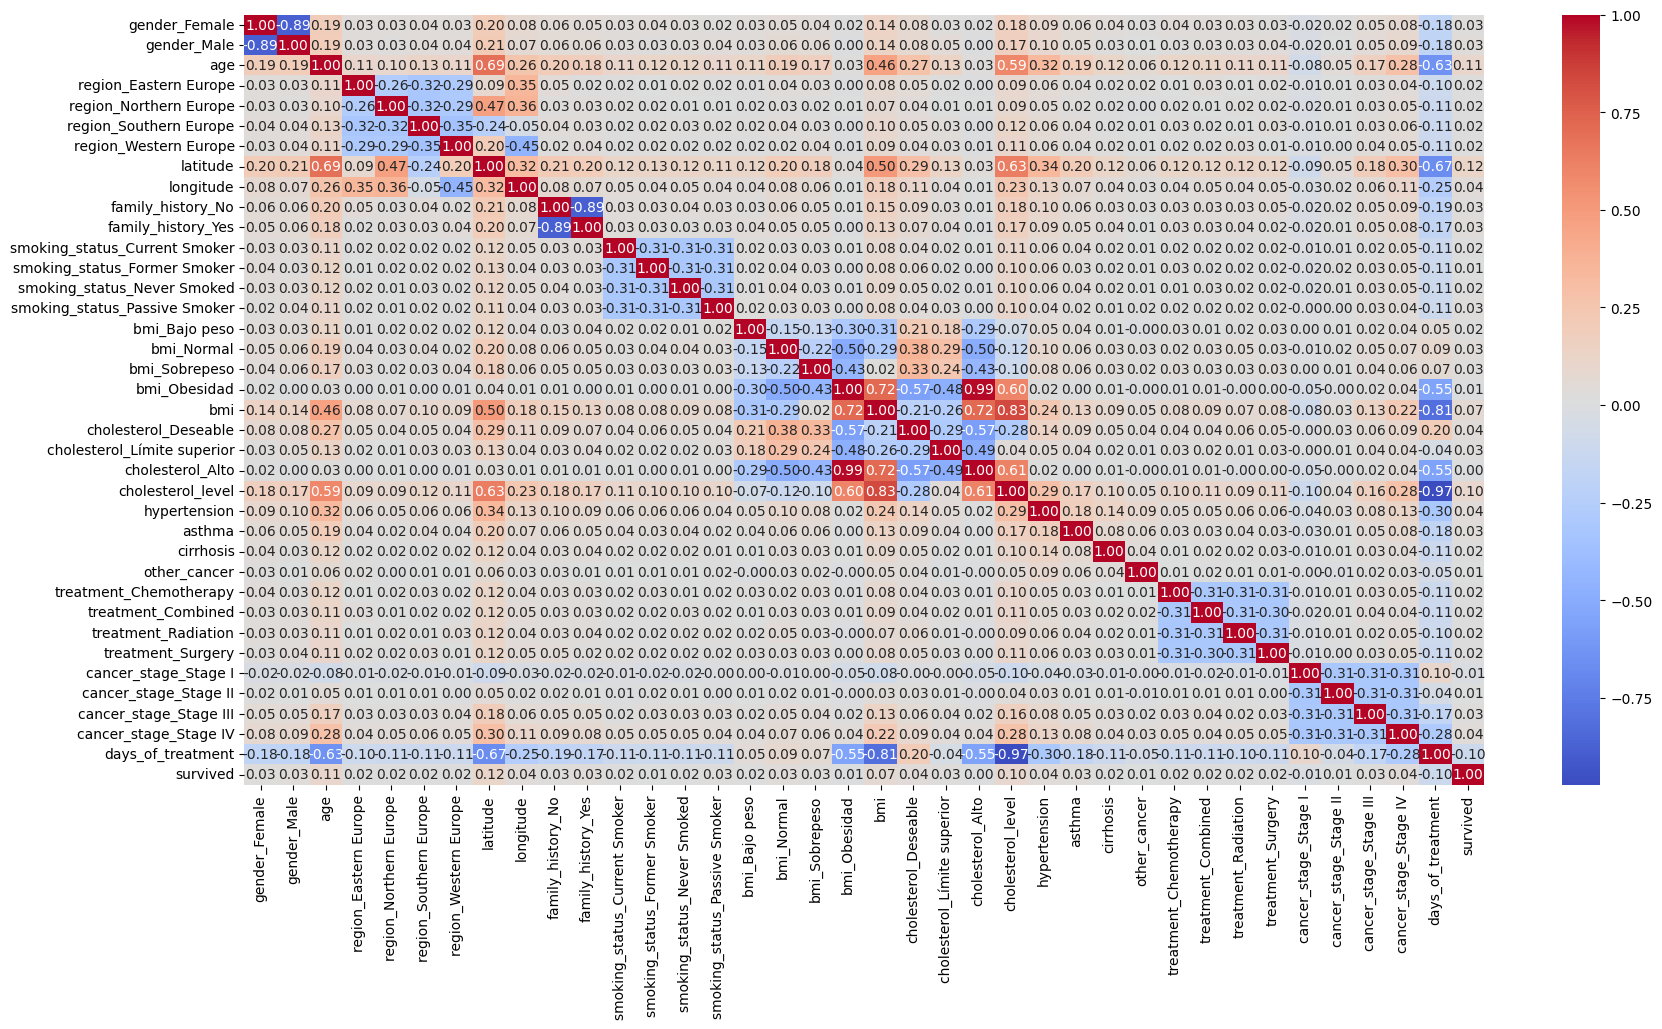
\includegraphics[width=\linewidth]{imagenes/MatrixCorrelacion.png}
    \caption{Matriz de Correlación}
    \label{fig:correlacion}
\end{figure}


\section{Diseño Visual}
En este capítulo, se describe el diseño visual desarrollado para explorar la influencia de diferentes variables en el cáncer de pulmón. El diseño se centra en tres tareas principales (T1, T2, T3), y cada una se apoya en componentes visuales específicos que permiten un análisis interactivo y detallado de los datos.

\begin{itemize}
\item T1:
Para comprender los factores que influyen en el cáncer de pulmón, se utilizan gráficos de correlación, diagramas de dispersión, y visualizaciones de importancia de variables. Estos componentes permiten observar las relaciones entre variables, como el estado de tabaquismo, el historial familiar, y el índice de masa corporal (BMI) con la probabilidad de desarrollar cáncer de pulmón.

\begin{itemize}
    \item \textbf{Gráfico de Correlación}: Muestra la relación entre las variables continuas, como la edad, el nivel de colesterol, y el índice de masa corporal (BMI), con la variable de supervivencia.
    \item \textbf{Gráfico de Importancia de Variables}: Este gráfico de barras destaca las variables categóricas y numéricas más influyentes en la predicción de la supervivencia o la etapa del cáncer.
    \item \textbf{Diagrama de Dispersión}: Permite explorar la influencia de variables geográficas (latitud y longitud) y otras variables numéricas en el diagnóstico de cáncer de pulmón.
\end{itemize}

\item T2:
El análisis de diferencias entre pacientes y los comportamientos de los distintos grupos se visualiza mediante mapas, gráficos de barras apiladas y diagramas de caja (box plots). Estos componentes permiten segmentar a los pacientes según diferentes criterios y observar patrones en sus comportamientos y características.

\begin{itemize}
    \item \textbf{Map View}: Un mapa interactivo que permite visualizar la distribución geográfica de los pacientes diagnosticados, mostrando la prevalencia por regiones y correlacionándola con variables de riesgo como el historial familiar y el estado de tabaquismo.
    \item \textbf{Gráfico de Barras Apiladas}: Este gráfico se utiliza para comparar la distribución de diferentes estados de tabaquismo y su relación con la supervivencia en las distintas regiones.
    \item \textbf{Box Plots}: Utilizados para comparar distribuciones de edad, nivel de colesterol, y BMI entre los distintos estadios del cáncer, proporcionando una visión clara de las diferencias entre los grupos de pacientes.
\end{itemize}

\item T3:
La distribución de las variables principales y su influencia en el cáncer de pulmón se visualiza mediante histogramas, gráficos de densidad, y diagramas de violín. Estos componentes ayudan a entender cómo se distribuyen las variables clave y su impacto en la enfermedad.

\begin{itemize}
    \item \textbf{Histogramas}: Permiten visualizar la distribución de la edad, BMI, y nivel de colesterol, mostrando cómo se agrupan los pacientes en diferentes categorías de riesgo.
    \item \textbf{Gráficos de Densidad}: Muestran la distribución suave de variables continuas, como la edad o la duración del tratamiento, destacando las áreas de mayor concentración de casos.
    \item \textbf{Diagramas de Violín}: Combinan información de la densidad de probabilidad con estadísticas descriptivas, ofreciendo una visión completa de la distribución de variables como la edad y el nivel de colesterol entre los diferentes estadios del cáncer.
\end{itemize}

\end{itemize}

Se ha diseñado una aplicación visual interactiva que incorpora los componentes mencionados para responder a las tareas de diseño:

\begin{enumerate}
    \item \textbf{Panel de Correlación}: Permite seleccionar variables y explorar sus correlaciones con la supervivencia y otras variables clave.
    \item \textbf{Vista Geográfica (Map View)}: Ofrece un mapa interactivo que muestra la distribución de los pacientes según la región y permite filtrar por diferentes factores de riesgo.
    \item \textbf{Panel de Distribución}: Facilita la visualización de distribuciones de variables principales mediante histogramas y gráficos de densidad.
\end{enumerate}

En la tabla \ref{tab:visualtareas} se presenta un cuadro que cruza los componentes visuales con las tareas de diseño.

\begin{table}[h!]
\centering
\caption{Componentes Visuales y Tareas de Diseño}
\begin{tabular}{|c|c|c|c|}
\hline
\textbf{Componente Visual} & \textbf{T1} & \textbf{T2} & \textbf{T3} \\ \hline
Gráfico de Correlación & X &  &  \\ \hline
Gráfico de Importancia & X &  &  \\ \hline
Diagrama de Dispersión & X &  &  \\ \hline
Map View &  & X &  \\ \hline
Gráfico de Barras Apiladas &  & X &  \\ \hline
Box Plots &  & X &  \\ \hline
Histogramas &  &  & X \\ \hline
Gráficos de Densidad &  &  & X \\ \hline
Diagramas de Violín &  &  & X \\ \hline
\end{tabular}
\label{tab:visualtareas}
\end{table}


\section{Resultados}

\section{Discusión}

\subsection*{T1: Factores que influyen en el cáncer pulmonar}

\begin{itemize}
    \item \textbf{¿Qué factores influyen en el diagnóstico del cáncer pulmonar?}
    \begin{itemize}
        \item Los factores que influyen en el diagnóstico del cáncer pulmonar incluyen la edad, el género, el historial de tabaquismo, el índice de masa corporal (BMI), el nivel de colesterol, la historia familiar de cáncer y el estadio de la enfermedad. Estos factores pueden proporcionar pistas importantes sobre la probabilidad de desarrollar cáncer pulmonar y ayudar en la detección temprana.
    \end{itemize}

    \item \textbf{¿Cómo afectan estos factores al diagnóstico de pacientes?}
    \begin{itemize}
        \item La edad y el historial de tabaquismo son factores de riesgo significativos para el cáncer pulmonar. El género puede influir en la prevalencia y el tipo de cáncer pulmonar. Un BMI elevado o un nivel de colesterol alterado también pueden estar asociados con un mayor riesgo de cáncer. La historia familiar de cáncer puede aumentar la predisposición genética al cáncer. El estadio de la enfermedad es crucial para determinar la extensión del cáncer y las opciones de tratamiento. La interacción de estos factores puede influir en la precisión del diagnóstico y en la decisión sobre el mejor enfoque terapéutico.
    \end{itemize}

    \item \textbf{¿Por qué algunos factores tienen un impacto más significativo que otros en el diagnóstico de la enfermedad?}
    \begin{itemize}
        \item Algunos factores, como el historial de tabaquismo y la edad, tienen un impacto más significativo debido a su fuerte correlación con el desarrollo del cáncer pulmonar. El tabaquismo es un factor de riesgo conocido y bien documentado, mientras que la edad puede reflejar la acumulación de exposiciones y daños a lo largo del tiempo. Otros factores, como el BMI y el nivel de colesterol, pueden tener un impacto más modesto pero aún relevante, ya que pueden estar asociados con la salud general y otros riesgos que contribuyen al cáncer.
    \end{itemize}
\end{itemize}

\subsection*{T2: Análisis de pacientes con diagnósticos y comportamiento}

\begin{itemize}
    \item \textbf{¿Cómo varían los comportamientos y patrones entre pacientes con diferentes diagnósticos de cáncer pulmonar?}
    \begin{itemize}
        \item Los comportamientos y patrones pueden variar significativamente entre pacientes con diferentes diagnósticos de cáncer pulmonar. Por ejemplo, pacientes diagnosticados en etapas tempranas pueden presentar síntomas menos graves y una mejor respuesta al tratamiento en comparación con aquellos diagnosticados en etapas avanzadas. Los patrones de comportamiento, como el historial de tabaquismo, pueden diferir entre los grupos y afectar el progreso de la enfermedad.
    \end{itemize}

    \item \textbf{¿Existen diferencias notables en el pronóstico y evolución entre distintos grupos de pacientes?}
    \begin{itemize}
        \item Sí, existen diferencias notables en el pronóstico y la evolución entre los distintos grupos de pacientes. Pacientes con diagnósticos en etapas más tempranas suelen tener un pronóstico más favorable y una mayor tasa de supervivencia en comparación con aquellos en etapas avanzadas. Además, el tipo de cáncer pulmonar (por ejemplo, cáncer de células no pequeñas frente a cáncer de células pequeñas) también puede influir en el pronóstico y la respuesta al tratamiento. Los factores genéticos y ambientales también juegan un papel en la variabilidad del pronóstico.
    \end{itemize}
\end{itemize}

\subsection*{T3: Distribución de variables clave}

\begin{itemize}
    \item \textbf{¿Cuál es la distribución de las variables principales en los pacientes con cáncer pulmonar?}
    \begin{itemize}
        \item La distribución de variables como la edad, el historial de tabaquismo, el BMI, y los niveles de colesterol en pacientes con cáncer pulmonar muestra una variabilidad significativa. Por ejemplo, la mayoría de los pacientes diagnosticados con cáncer pulmonar pueden tener un historial de tabaquismo prolongado y presentar un rango de edades avanzadas. La distribución del BMI y los niveles de colesterol puede variar, pero también puede mostrar tendencias relacionadas con el estado de salud general de los pacientes.
    \end{itemize}

    \item \textbf{¿Cómo influye esta distribución en la dinámica y el tratamiento del cáncer pulmonar?}
    \begin{itemize}
        \item La distribución de estas variables influye en la dinámica del cáncer pulmonar al proporcionar información sobre los factores de riesgo predominantes y ayudar a identificar patrones en la progresión de la enfermedad. Esta información puede guiar el enfoque del tratamiento, ya que diferentes perfiles de pacientes pueden requerir diferentes estrategias de manejo. Por ejemplo, pacientes con un historial de tabaquismo intenso pueden ser tratados con enfoques específicos para abordar los riesgos asociados con el tabaquismo. La comprensión de la distribución de variables clave también ayuda en la personalización del tratamiento y la identificación de posibles factores predictivos para la evolución de la enfermedad.
    \end{itemize}
\end{itemize}
\section{Conclusion}
Los análisis visuales presentados en las figuras sugieren una relación significativa entre el índice de masa corporal (BMI), los niveles de colesterol y la probabilidad de desarrollar cáncer pulmonar u otros tipos de cáncer. Específicamente, personas con un BMI elevado y colesterol alto muestran una mayor susceptibilidad a encontrarse en estados avanzados de cáncer. Estos hallazgos subrayan la importancia de monitorear el colesterol y el BMI como posibles indicadores de riesgo, sugiriendo que aquellos con niveles altos deberían considerar la realización de chequeos preventivos de cáncer para una detección temprana y un manejo adecuado.


Según la \autoref{fig:tsne_cholesterol}, podemos demuestran que una persona con nivel de colesterol superior debería someterse a un chequeo preventivo de cáncer, porque presenta una mayor probabilidad de desarrollar  cáncer pulmonar. Según la \autoref{fig:tsne_bmi}, se observa que el índice de masa corporal (BMI) tiene una correlación con los resultados mostrados en la  \autoref{fig:tsne_cancer_stage} ya que las personas con mayor BMI tienden a tener niveles más altos de colesterol. Además, la  \autoref{fig:tsne_cancer_stage} revela que las personas con obesidad y colesterol alto tienen una mayor probabilidad de encontrarse en algún estado avanzado de cáncer. Asimismo, en la \autoref{fig:tsne_other_cancer} se muestra que estas mismas personas también pueden tener una mayor susceptibilidad a desarrollar otros tipos de cáncer.

El análisis revela que los factores demográficos y médicos, como la edad, el género, el estado de tabaquismo, el índice de masa corporal (BMI), el nivel de colesterol, la historia familiar de cáncer y el estadio de la enfermedad, tienen un impacto significativo en la supervivencia de los pacientes con cáncer pulmonar. Sin embargo, a pesar de los avances en técnicas de visualización y análisis, la complejidad de las interacciones entre estos factores aún no está completamente entendida. La falta de comprensión detallada de estas interacciones subraya la necesidad de modelos predictivos más precisos y estrategias de tratamiento más efectivas. Además, la propuesta de utilizar técnicas de reducción de dimensionalidad, como PCA, para mejorar la precisión del modelo destaca la importancia de abordar problemas de desequilibrio en los datos y mejorar la efectividad de los clasificadores en el contexto de datos médicos.



\appendices
\section{Colab TrabajoCancerPulmon v2.ipynb}
Detalle de la aplicación
\begin{itemize}
  \item Lenguaje de Programación: Python
  \item Servidor: Google
  \item Librerias Principales; sklearn, matplotlib, pandas,seaborn, numpy
\end{itemize}
\href{https://colab.research.google.com/drive/1-HcDMOWJxGsakeZxqYCUc18EXPyz__4q?usp=sharing}{URL: Código  colab.research.google }

\section{GitHub}
Url de git hub:
\href{https://github.com/hAriasm/RecuperacionInfo}{URL: RecuperacionInfo }

 \section{Video explicativo}
Url de Youtube:
\href{https://github.com/hAriasm/RecuperacionInfo}{URL: Youtube }



\ifCLASSOPTIONcaptionsoff
  \newpage
\fi

\begin{thebibliography}{1}

\bibitem{IEEEhowto:kopka}
H.~Kopka and P.~W. Daly, \emph{A Guide to {\LaTeX}}, 3rd~ed.\hskip 1em plus
  0.5em minus 0.4em\relax Harlow, England: Addison-Wesley, 1999.

\bibitem{ferraz2017}
R.~O.~Ferraz and D.~C.~Moreira-Filho, ``Análise de sobrevivência de mulheres com câncer de mama: modelos de riscos competitivos,'' \emph{Ciência \& Saúde Coletiva}, vol.~22, no.~11, pp.~3743--3754, Nov. 2017. [Online]. Available: https://doi.org/10.1590/1413-812320172211.05092016.

\bibitem{arxiv14031949}
Author(s) Name, "An Analysis of Machine Learning Models for Efficient Data Processing," \textit{International Journal of Computer Applications}, vol. 77, no. 3, pp. 33--38, 2013. [Online]. Available: \href{https://doi.org/10.48550/arXiv.1403.1949}{DOI: 10.48550/arXiv.1403.1949}.

\bibitem{jolliffe2016pca}
I.~T. Jolliffe and J.~Cadima, ``Principal component analysis: a review and recent developments,'' \emph{Philosophical Transactions of the Royal Society A: Mathematical, Physical and Engineering Sciences}, vol. 374, no. 2065, p. 20150202, 2016.

\bibitem{maaten2008tsne}
L.~van~der Maaten and G.~Hinton, ``Visualizing data using t-{SNE},'' \emph{Journal of Machine Learning Research}, vol.~9, pp. 2579--2605, 2008.

\bibitem{olsson1979maximum}
U.~Olsson, ``Maximum likelihood estimation of the polychoric correlation coefficient,'' \emph{Psychometrika}, vol.~44, no.~4, pp. 443--460, 1979.


\bibitem{aha_colesterol}
American Heart Association (AHA), ``Guideline on the Treatment of Blood Cholesterol to Reduce Atherosclerotic Cardiovascular Risk in Adults,'' \emph{American College of Cardiology}, 2018. [Online]. Available: https://www.heart.org/en/professional/education/guidelines-for-treatment-of-blood-cholesterol

\bibitem{cdc_bmi}
Centers for Disease Control and Prevention (CDC), ``Defining Adult Overweight and Obesity,'' \emph{CDC}, 2020. [Online]. Available: https://www.cdc.gov/obesity/adult/defining.html

\bibitem{nih_bmi_colesterol}
National Institutes of Health (NIH), ``Clinical Guidelines on the Identification, Evaluation, and Treatment of Overweight and Obesity in Adults,'' \emph{NIH}, 1998. [Online]. Available: https://www.nhlbi.nih.gov/files/docs/guidelines/obesity.pdf

\bibitem{hunter2007matplotlib}
Hunter, J. D. (2007). Matplotlib: A 2D graphics environment. \textit{Computing in Science \& Engineering}, 9(3), 90-95. doi:10.1109/MCSE.2007.55


\bibitem{pedregosa2011scikit}
Pedregosa, F., Varoquaux, G., Gramfort, A., Michel, V., Thirion, B., Grisel, O., ... \& Duchesnay, É. (2011). Scikit-learn: Machine learning in Python. \textit{Journal of Machine Learning Research}, 12, 2825-2830.


\end{thebibliography}


\end{document}


